%! Author = andrei.olar@ubbcluj.ro
%! Date = 03.09.2023

% Preamble
\documentclass[11pt]{article}

% Packages
\usepackage{amsfonts}
\usepackage{amsmath}
\usepackage{amsthm}
\usepackage{enumitem}
\usepackage{hyperref}
\usepackage{xcolor}
\usepackage{cite}
\usepackage{array}
\usepackage{graphicx}
\graphicspath{ {./img/} }

% Document
\begin{document}
    \theoremstyle{definition}
    \newtheorem{defn}{Definition}[section]
    
    \section{Abstract}\label{sec:abstract}


    \section{Introduction}\label{sec:introduction}
    Entity resolution is the task of finding out whether two pieces of
    information refer to the same real-world item or not.
    There's more restrictive definitions of entity resolution as the task of
    identifying and linking representations of data from two or more
    sources\cite{Qia17}.
    We share the opinion that identifying and linking data consitutes a more
    specialized process\cite{Tal11}.
    The task of gathering information about a generic pound of potatoes across
    various markets is still an entity resolution task, in our view.
    
    Probably because of its generic nature, entity resolution also goes by many
    different names such as: record linkage, data deduplication, merge-purge,
    named entity recognition, entity alignment or entity
    matching\cite{Tal11,fever2009}.

    Entity resolution has many practical applications ranging from linking
    medical records to doing background checks on persons of interest to 
    identifying plagiarism.
    As an aside, combining information from different media (sound, images,
    motion, smell, etc) is also a form of entity resolution and opens up many
    avenues into its future as an area of study.

    The glue that binds all of the above examples has at least the following
    ingredients:
    \begin{itemize}
        \item\textit{a concern for a real-world entity}, for if the task were
        not about a something from our world, the resolution would not have a
        clear goal;
        \item\textit{no implication as to the used method}, because if we
        stipulated a certain way to perform entity resolution, we might not be
        able to;
        \item\textit{the representation of information is computer friendly},
        because if it weren't, it might not be possible to study the task by
        means of computer science.
    \end{itemize}

    We must clarify regarding the concern for a real-world entity that entity
    resolution tasks do not deal with real-world entities directly but with
    information about them\cite{Tal11}.
    In other words, entity resolution tasks typically don't know about the
    real-world objects or entities they are meant to resolve\cite{Chen09}.
    Naturally, entity resolution tasks will not perform perfectly from a
    qualitative standpoint.
    We are interested to find common ground for measuring entity resolution
    performance.
    
    Historically, entity resolution performance was measured in many ways, some
    of which (true positive rate, false positive rate) have been contested for
    certain use cases\cite{Goga2015}.
    Our work means to standardize qualitative entity resolution quality
    measurement across the board.
    We base our methodology on the mathematical models that underpin entity
    resolution tasks.

    The first sections of this paper go over the contributions it makes and the
    work related to this paper.
    Afterwards we start our journey towards the main subject by introducing some
    basic entity resolution terminology which is used throughout the paper.
    Following that, we describe the scientific problem of comparing the
    performance of entity resolution tasks.
    Next we go through three classical mathematical models and show how each of
    them influences entity resolution evaluation.
    After the conceptual framework is ready, we provide experimental data to see
    how the concepts map to practice.
    In the closing sections, we provide some insights that we are now able to 
    glean from the results, draw some conclusions and finally hint towards
    future work on this topic.

    \section{Contributions}\label{sec:contributions}

    This paper makes the following contributions:

    \begin{itemize}
        \item materializes the connection between mathematical model and entity
        resolution task
        \item provides a generic framework for measuring the qualitative
        performance of entity resolution tasks
        \item introduces a software system that uses this framework
    \end{itemize}

    \section{Related Work}\label{sec:related}
    
    Because of the generality of the topic, there is much existing work that
    relates in some way or another to this paper.
    However, three categories of papers share the most concerns with this one:
    entity resolution system presentations, syntheses of theoretical models for
    entity resolution and syntheses of evaluation metrics for entity resolution.

    The papers that introduce entity resolution systems relate to this one
    through the shared goal of generalizing how entity resolution tasks are run
    and, therefore, evaluated.
    Most of the systems referenced here provide at least a few generic metrics
    to evaluate entity resolution performance.
    They 

    At the dawn of the 21st century, FEBRL\cite{febrl2002} emerged as one of the
    first extensible systems to tackle measuring entity resolution performance.
    It was succeeded by FEVER\cite{fever2009} and OYSTER\cite{oyster2012}. 
    These systems have all paved the way to generalizing our understanding about
    entity resolution and to ever more improvements in the quality of entity
    resolution tasks.
    Later on, systems like `Papers with Code'\cite{papwithcode2019} brought in
    a social dimension to how we compare the qualitative performance of entity
    resolution tasks.
    Newer systems resemble frameworks more than they resemble
    applications\cite{magellan2020,jedai2017}.
    These systems are open-source and encourage social collaboration around
    entity resolution, too.
    
    There exist numerous syntheses on the theoretical models for entity
    resolution\cite{fs1969,Ben2009Swoosh,Tal11}.
    Some of the available models have been compared and
    explained\cite{Tal11,tal2013}.

    Ways in which entity resolution tasks are similar even though they seem
    to have nothing in common have been discussed in papers that deal with
    certain steps of the entity resolution process\cite{Pap19,Chen09}.

    \section{Terminology}\label{sec:terminology}

    Given that we have just reserved the term ``entity'' for real-world items,
    we have to come up with new terms for the concepts used in the context of
    entity resolution.
    We start by saying that entity resolution operates on information sources.

    \begin{defn}
        An \textit{information source} represents a sequence of decoded messages
        that originate somewhere and can be processed by the entity resolution
        task which reads them over a communication channel.
    \end{defn}

    The terms `decoded', `message' and `communication channel' refer to concepts
    from the field of information theory\cite{ash2012it}.
    
    An entity resolution task can operate on one or multiple information
    sources.
    Information sources may be bounded (such as files or databases) or unbounded
    (such as streams).
    
    In the context of the above definition, the entity resolution task is the
    computer program doing the processing.
    What sets entity resolution programs apart is the notions they use to
    process information from a particular source.

    \begin{defn}
        An \textit{attribute} is information about an entity that has a certain
        meaning in a context given by a frame of reference and certain rules of
        interpretation.
    \end{defn}

    Attributes by themselves are not enough to describe an entity.
    For example, `red' fully describes an entity only if we are looking for
    colors.
    If we're looking for fruit, `red' is only one of several attributes that
    help describe fruit.
    For example we might be interested in `sour' or `sweet' as well as in
    `small', `medium' or `large'.

    \begin{defn}
        An \textit{entity reference} is a collection of attributes that refer
        to a real-world entity which can be formed by following an organizing
        principle (or order) of the information source where the attributes are
        all located.
    \end{defn}

    The organizing principle of an information source is simply an order that
    facilitates processing that information source.
    For example, in a CSV file it would be the rule that up until the first
    comma on each line we should find a color value.
    For operations on databases such as joins, the organizing principles is
    built around data records.
    For named entity recognition, the organizing principle is built around
    mentions.

    A good generalization of the notions in the above examples put in the
    context of entity resolution might be that of a
    \textit{reference}\cite{Ben2009Swoosh}.
    For in this context the rules for processing records, mentions or lines in
    CSV files are used simply to find references to real-world entities.

    The organizing principle of an information source shouldn't be confused with
    the structure of the information in that source.
    A single table record in a database might have a few attribute that
    reference one entity (for example a company or a person) and a few other
    attributes that reference another entity (a building).
    For entity resolution tasks that value geolocation above other things, the 
    fields that reference the building will constitute the entity reference.
    For tasks that identify people, the entity reference will be comprised from
    the attributes that reference a person or a company.
    The organizing principle of the information source by which attributes are
    collected as entity references by the entity resolution task is extrinsic to
    the information source and is somehow linked to the entity resolution task
    itself.
    We say `linked' because the organizing principle may or may not be an
    integral part of the entity resolution task.
    For instance, entity alignment tasks rely on external knowledge bases and
    entity matchers based on deep learning rely on machine learning for
    determining the organizing principle of every data source they consume.

    The other important distinction is that the attributes that make up an
    entity reference are collected from the same information source.
    This creates a clear belonging relationship between entity reference and
    information source.
    
    Let's suppose that we are looking to identify colors across multiple
    information sources.
    In one information source the colors are represented as `red', `green' or 
    `blue'.
    In another information source they are represented as `CC0000', `00CC00' or
    `0000CC'.
    Because we are looking for colors we decide that our organizing principle
    should dictate that references contain only one attribute.
    However, up until now we haven't articulated a way to tell the entity
    resolution task that.
    Namely: how do we tell the entity resolution task that it's looking for
    something that is a \textit{color}.
    Or, formulated as a question: what is \textit{color}?

    \begin{defn}
        A \textit{trait} is a semantic rule that guides the entity resolution
        task in recognizing the organizing principle of each information source
        that it uses as input.
    \end{defn}

    Every entity resolution task has goals it must accomplish.
    Some tasks stitch news articles together, others help organize content
    across social networks or deduplicate the information stored in database
    tables.
    For each task there are rules of interpreting the information at hand that
    stand out above others.
    In our case, we must simply tell our task that it should be interested only
    in colors and how those colors might look like depending on information
    source.
    
    The notion that's the most similar to that of a trait is the `feature':
    \textit{an individual measurable property or characteristic of a
    phenomenon}\cite{bishop2006pattern}.
    The mechanics of how traits and features function is near identical.
    The difference between a trait as defined here and a feature is a matter of
    perspective.
    Features are part of a more objective perspective on information.
    Traits as they are defined here are concerned with the contextual meaning of
    things.
    In the broadest sense, they are nothing more than algorithms that extract
    information according to the subjective goal of the entity resolution task.
    A trait can help the entity resolution task extract one or more attributes
    for a given entity reference that can't be inferred from the underlying
    information alone.
    For example, a trait called `profitable' is different from a physical
    representation in the form of a table column or a JSON property.
    Imagine an entity resolution task that is meant to find companies across
    databases.
    One of the traits this entity resolution task is looking for is the company
    profitability.
    In a database table, it looks at values stored in a column called `profit'.
    In a no-SQL collection, it looks at the values stored under the
    `isProfitable' property.
    Yet, the entity resolution task simply looks for the `profitable' trait in
    both these information sources to help shape the entity references it finds.

    To sum up, an attribute of an entity reference always exists in an
    information source, whereas a trait of the entity resolution task does not.
    Entity resolution tasks extract attributes that they assign to entity
    references based on the traits specific to each task.
    This point of view is supported by the need to design entity resolution
    systems that are extensible based on their sources of
    information\cite{fever2009}\cite{magellan2020}\cite{oyster2012}.

    So far we have not discussed what happens if entity references point to the
    same real-world entity.
    
    \begin{defn}
        The logical group of entity references that point to the same real-world
        entity according to the entity resolution task's parameters is known as
        the \textit{entity profile} of that real-world entity within the entity
        resolution task.
    \end{defn}

    It is important to understand that the entity profile and the real-world
    entity are not the same.
    The entity profiles are simply manifestations of the input parameters of the
    entity resolution task (namely the information sources and the traits) and
    they represent the output of the entity resolution task.
    
    By using the terms \textit{information source}, \textit{attribute},
    \textit{trait}, \textit{entity reference} and \textit{entity profile} we can
    finally define the entity resolution problem.

    \section{Problem Definition}\label{sec:problem}

    In a broad sense, the entity resolution process is usually comprised of four
    different activities\cite{Pap19,Tal11}:
    \begin{itemize}
        \item \textit{entity reference extraction} --- the first phase of entity
        resolution deals with extracting entity references from multiple
        sources, as detailed in the introduction of this paper;
        \item \textit{blocking} and \textit{filtering} --- at this stage, the
        entity resolution task groups in the same `block' entities that share
        similar traits and then within each block all entities that can't
        possibly match are filtered \textit{out}; the intent here is to allow
        entity resolution tasks to work with large amounts of data \cite{Pap19};
        \item \textit{matching} --- one of the defining activities of the entity
        resolution process and compares entity references to one another;
        \item \textit{clustering} --- the other defining activity within the
        entity resolution process whereby matching references are collected
        together in entity profiles.
    \end{itemize}

    In a stricter sense, by entity resolution we usually mean the latter two
    stages of the entity resolution process.
    Although our concern is with entity resolution evaluation and the comparison
    of entity resolution processes, we can't overlook the extraction process
    because this process defines the data structures that are used throughout
    the entire entity resolution process.

    Given:
    \begin{itemize}
        \item $n \in N^*$ pairs (($S_i$, $n_i$), $1 \leq i \leq n$, $n_i \in N$), 
        where $S_i$ is an information source and $n_i$ is the number of messages
        in $S_i$,
        \item $m_i \in N^*$ traits, ($t_{ij}$, $1 \leq j \leq m_i$) for each
        information source $S_i$ so that
        \item each trait $t_{ij}$ can generate at most $a_{ij} \in N^*$
        attributes,
    \end{itemize}
    an entity resolution task $ER$ applies each trait $t_{ij}$ onto the source
    $S_i$, ($1 \leq i \leq n$, $1 \leq j \leq m_i$), in order to extract
    $r_{{S_i}k}$ entity references where
    ($0 \leq k \leq n_i \cdot \sum^{m_i}_{j=1}a_{ij}$).
    We denote with $R$ the domain of all the $r_{{S_i}k}$ entity references that
    were extracted by $ER$.
    Similarly, we denote with $P$ the domain of all entity profiles.
    The matching and clustering steps of the $ER$ task can be combined in a
    single function $E: R \rightarrow P$ that converts individual references to
    entity profiles.
    The exact definition of this function is specific to the mathematical model
    that underpins the entity resolution process.
    The data representation of the entity profiles in $P$ also varies according
    to the mathematical model of choice.
    On the other hand, the abstract data types used for representing the
    concepts that are part of building $R$ are invariant.

    The most basic building block in the context of entity resolution is the
    humble attribute.
    We denote with $A$ the domain of all possible attributes that can be used by
    the task $ER$ described above.

    In this context, let $r_{{S_i}{k_j}}$ denote the $k_j$th ($1 \leq j \leq k$)
    entity reference extracted from the source $S_i$.
    Then $r_{{S_i}{k_j}}$ is always represented as a tuple
    ($a_r$, $r \in N^*$, $a_r \in A$), $r_{{S_i}{k_j}} \in A^r$.
    Note that $r$ varies for each $k_j$.
    The concept of an order external to the information source and the manner in
    which we defined traits serves as the reason why tuples express entity
    references sufficiently well.

    A trait is then a function that helps construct entity references.
    The definition domain of this function materializes only when the $ER$ task
    extracts a given entity reference $r_{{S_i}{k_j}}$.
    The domain of this function is then the domain of all of the attributes in
    the source $S_i$ that could be meaningful in the context of constructing the
    entity reference $r_{{S_i}{k_j}}$ from a certain subjective perspective.
    We denote this domain with $A_{{S_i}{k_j}}$.
    Then the trait is defined as a function $t: S_i \rightarrow A^x$, where
    $x \in N^*$ and $x$ varies with $k_j$ as defined above for entity
    references.
    This formal definition of the trait satisfies the needs of any extraction
    process specific to entity resolution.

    During the extraction process, the entity resolution task applies multiple
    traits with the end result of building the domain of entity references:

    \[
        Ref = \bigcup_{i \in N^*,1 \leq j \leq k} r_{{S_i}{k_j}}
        \textrm{, with r, S and k specified above}
    \]

    The $Ref$ domain is constructed through entity reference extraction and
    after the entities have been extracted, we are no longer concerned with the
    input information sources.
    Another observation is that every type of entity resolution task can be made
    to work on such an input domain\cite{Pap19}.
    A task that uses two or more input sources can be reduced by concatenating
    entity references extracted from those sources.
    So, every entity resolution task can be viewed at its core as either a
    data deduplication or a clustering task.
    Regardless of the optics, the input domain contains only entity references.
    In our view, the entity resolution task is agnostic of the provenance of the
    entity references it processes.
    
    That allows us to formalize the entity resolution task as a function:
    \[
        e : Ref \rightarrow \{P_x \mid x \in \mathbb{N}, P_x \in P \},
    \]
    
    where $P$ is the domain of entity profiles and $x$ is the number of
    resulting entity profiles.
    We denote with $Res=\{P_x \mid x \in \mathbb{N}, P_x \in P\}$ as the domain
    of all entity resolution task results.
    Note that $Res$ \textit{is a set} because the nature of the entity
    resolution task is to cluster or deduplicate, both operations being widely
    understood as operations that result in creating unique items (be they
    clusters or unique entity references).

    It stands to reason that the domain $Res$ contains a result which is the
    closest to our understanding of the real world from a given perspective in
    a given context.

    \begin{defn}
        We define the \textit{ground truth} $G$ of an input entity reference
        domain $Ref$ the entity resolution result comprised of entity profiles
        such that
        $\{P_g \mid g \in N\textrm{, $P_g$ describes a real-world entity
        completely}\}$.
    \end{defn}

    In other words the ground truth is the ideal entity resolution result for 
    given input data, but in a given context, from a given perspective.
    This result contains only those profiles that describe real-world entities.

    Now that we know what the ideal result of an entity resolution task looks
    like, we can at least formulate a measure of the task's relative qualitative
    performance with respect to the ground truth of the task's input.
    
    \begin{defn}
    Given an entity resolution task $e: Ref \rightarrow Res$ and the ground
    truth $G$ for the input entity reference domain $Ref$, a \textit{quality
    metric} is an idempotent function $q: Res \rightarrow \mathbb{R}$ that
    measures the similarity between the input of the function and $G$.
    \end{defn}

    In practice, we should strive to implement quality metric as \textit{pure}
    functions in the sense that running them on a computer will not entail any
    side-effects.

    As stated before, the shape and structure of the items in $Res$, including
    $G$, depends on the mathematical model underpining a specific entity
    resolution task implementation.
    Because the input domain of the quality metrics changes according to the
    used mathematical model, the set of quality metrics available for describing
    the performance of a certain entity resolution task $Q = \{q_y \mid y \in
    \mathbb{N}\}$ is dependent on the mathematical model used for implementing
    that task.

    \subsection[ere]{Entity Resolution Evaluation}\label{sec:ere}

    In the strictest sense, comparing two entity resolution tasks is possible as
    long as they can be evaluated using the same set $Q$ of qualitative
    evaluators.
    Note that if the entity resolution $e_1$ can be evaluated using a set of
    quality metrics $Q_1$ and $e_2$ can be evaluated using a set of quality
    metrics $Q_2$ such that $Q_1 \cap Q_2 \neq \emptyset$, we have a set of
    quality metrics $Q_\cap = Q_1 \cap Q_2$ that allows us to compare $e_1$ and
    $e_2$ based on $Q_\cap$.
    Future developments will seek to further loosen this constraint to allow
    comparing entity resolution tasks that do not share a set of qualitative
    evaluators.

    \subsection[cert]{Comparing Entity Resolution Tasks}\label{subsec:cert}

    Entity resolution tasks can be compared in quantitative terms without any
    issue.
    Metrics for the amount of hardware resources they consume or the physical
    time that elapses for a data set of a given size are invariant across the
    many possible implementations of entity resolution solutions.

    The problem of comparing entity resolution results from a qualitative
    perspective is significantly less clearly delimited.
    Each mathematical model is rooted in a different branch of mathematics and,
    as such, works with different assumptions and different expressions of the
    surrounding reality.
    For example, all statistical models express the real world in terms of
    probabilities.
    On the other hand, a construct of set theory will invariably explain the
    real world in terms of set operations, properties and it will use algebraic
    constructs.
    The comparison problem must take into account these limitations.

    \begin{defn}
        Given
        \begin{itemize}
            \item the set of entity references $Ref$,
            \item a set of quality metrics $Q$ that are common to all
            entity resolution tasks $e_i : Ref -> Res$, $i \in \mathbb{N}$
            \item the ground truth $G$ for the input domain $Ref$,
            \item the quality metric results
            $V_i=\{q_{i} \mid q_{i} = q(G, e_i), q \in Q\}, i \in \mathbb{N}$,
        \end{itemize}   
        we define the comparison of the entity resolution tasks above as
        $C : (
            \{V_i \mid i \in \mathbb{N}\}
            \times
            \{V_j \mid j \in \mathbb{N}\},
            i \neq j
        ) \rightarrow \{-1, 0, 1\}$ such that:
        \[ 
C(V_i, V_j) = \left\{
\begin{array}{ll}
      -1,~\textrm{if $e_i$ is less fit for purpose than $e_j$}\\
      0,~\textrm{if $e_i$ is as fit for purpose as $e_j$}\\
      1,~\textrm{if $e_i$ is better fit for purpose than $e_j$}\\
\end{array} 
\right. 
\]

    \end{defn}

    Quality metrics are specific to a mathematical model.
    
    \section[mm]{Mathematical Models}\label{sec:mm}

    The ground truth used for evaluating the performance of an entity resolution
    task and the entity resolution result are represented similarly.
    The representation depends on the mathematical model used by the entity
    resolution task.
    
    The mathematical models available for entity resolution range from ones
    based on complex networks and graph theory\cite{Li2020} to ones based on
    probabilities\cite{fs1969} or algebra\cite{Tal11,Ben2009Swoosh}.

    John R. Talburt already provides a description of these mathematical models
    in his book on entity resolution and information quality\cite{Tal11}.
    This paper aims to take a deeper look at how two of the models described in
    that book might be connected.

    \subsection[fsm]{Fellegi-Sunter Model}\label{subsec:fsm}

    In the late 1960s Ivan Fellegi and Alan Sunter wrote the seminal
    paper\cite{fs1969} for what they called record linkage and what would later
    become known as entity resolution.
    To this day, their mathematical model based on probability theory is the
    most popular way of formalizing the entity resolution problem.
    In this mathematical model, entity resolution is a function that aids in 
    probabilistic decision making.
    
    \subsubsection[fsm-desc]{Description}\label{subsec:fsm-desc}

    The original model defines record linkage as an operation over two input
    sets, $A$ and $B$.
    The result of the operation is a set containing pairs of items
    $X = \{(a, b), a \in A, b \in B\}$ or $X = A \times B$.
    
    The model then deconstructs $X$ to two disjoint subsets $X = M \cup U$: $M$ for pairs that
    contain matching items and $U$ for pairs that contain non-matching items.

    \begin{align}
        M &= \{(a, b) | a == b, a \in A, b \in B\}~\textrm{and} \\
        U &= \{(a, b) | a \neq b, a \in A, b \in B\}
    \end{align}

    The model proposes that if $a \in A$ and $b \in B$ are two vectors, their
    comparison will also be a vector denoted $\gamma \in \varGamma$, where
    $\varGamma$ denotes the set of all possible values of $\gamma$.
    The comparison between $a$ and $b$ is performed between each corresponding
    element in each of the two vectors.
    The elements of $\gamma$ vary according to the type of comparison that is
    performed\cite{winkler1990}.

    In this context, a match decision function can make one of three decisions
    regarding a pair from $X$ according to the F-S model:
    
    \begin{itemize}
        \item consider it a \textit{link ($A_1$)} between the items;
        \item consider it a \textit{non-link ($A_3$)} between the items, and
        \item leave things undecided, thus marking it as a \textit{possible link
              ($A_2$)}.
    \end{itemize}
    
    Then a linkage rule is a function $L:\varGamma \rightarrow D$,
    $D=\{d(\gamma)\}$, where
    
    \begin{align}
        &d(\gamma) = \{P(A_1|\gamma),P(A_2|\gamma),P(A_3|\gamma)\};
        &\textrm{so that}~\sum_{i=1}^{3}P(A_i|\gamma) = 1\nonumber.
        \gamma \in \varGamma\nonumber
    \end{align}

    In other words, for a $\gamma \in \varGamma$, $L(\gamma) = \{P(A_1|\gamma),
    P(A_2|\gamma), P(A_3|\gamma)\}$ so that the probabilities sum up to $1$.

    When using this model the purpose of entity resolution is to find the
    optimal linkage rule.
    The F-S theorem defines it as the linkage rule that minimizes
    $P(A_2|\gamma)$.
    In other words, the optimal linkage rule according to the F-S model is the
    linkage rule without uncertainties.
    This optimization inclination of the model makes it very well suited for
    both rule-based\cite{oyster2012} and machine learning\cite{deepm2020}
    implementations.
    
    In this universe, two conditional probabilities become interesting:

    \begin{align}
        m(\gamma)&=P(\gamma(a, b) | (a, b) \in M)~\textrm{and}\nonumber\\
        u(\gamma)&=P(\gamma(a, b) | (a, b) \in U)\textrm{.}\nonumber
    \end{align}

    \noindent
    $m(\gamma)$ is the probability of a $\gamma$ comparison vector given an
    $(a, b)$ \textit{link}.
    $u(\gamma)$ is the probability of a $\gamma$ comparison vector given an
    $(a, b)$ \textit{non-link}.
    For brevity, we have not used the complete notation pertaining to records
    from the original paper.

    The two probabilities outlined above are important because they help us
    express the probabilities of the Type I and Type II statistical errors
    associated with the decision function that sits at the core of the linkage
    rule definition above.
    The probabilities of the two types of error are expressed as:

    \begin{align}
        \mu&=\sum_{\gamma \in \varGamma}u(\gamma)P(A_1|\gamma)\textrm{,~and}\nonumber\\
        \lambda&=\sum_{\gamma \in \varGamma}m(\gamma)P(A_3|\gamma)\nonumber
    \end{align}

    where:

    \begin{itemize}
        \item $\mu$ represents the Type I error of items that were erroneusly
        linked (i.e pairs in $M$ that do not belong in $M$), and
        \item $\lambda$ represents the Type II error of items that were
        erroneously \textit{not} linked (i.e. pairs in $U$ that do not belong in
        $U$).
    \end{itemize}

    \subsubsection[fms-term]{Terminology Translation}\label{fsm-term}

    To link the Fellegi-Sunter model to our own terminology, let's start by
    talking about $a \in A$ and $b \in B$.
    The original F-S model calls $A$ and $B$ ``populations'' and $a$ and $b$,
    ``population elements''.
    A distinction is made between records, denoted with $\alpha(a)$ and
    $\beta(b)$, and population elements.
    Most of the original paper refers to records.

    It is safe for the reader to assume that in our terminology the population
    elements correspond to real-world entities and the records correspond to
    entity references.
    However, our view on $\alpha(a)$ and $\beta(b)$ is more broad in that we
    think of them not merely as records, but as functions that associate a
    representation as records(entity references) to the population elements
    (information about real-world entities).
    We used the notion of traits or extraction traits to express this concept.
        
    The $A$ and $B$ populations equate roughly to our notion of information
    sources.
    The ``population'' concept is a particularization of our information source
    concept because it is defined as a set in the original paper whereas our
    definition includes other possible data representations.
    The concept is also more general than our own concept because we defined
    information sources under the assumption of machines being able to process
    the information within them, whereas a population is a more general concept
    to which this restriction need not apply.

    The Fellegi-Sunter model works under the assumption that there are two
    populations $A$ and $B$ and defines the linkage rule as a function that uses
    conditional probabilities that involve both populations.
    On the other hand, our $Ref$ domain for entity references is clearly
    solitary.
    Using our terminology we would denote $A$ with $S_1$ and $B$ with $S_2$.
    We start constructing our $Ref$ domain by using traits to extract $n_1$
    entity references from $S_1$ and $n_2$ entity references from $S_2$.
    Then $Ref = \{r_{{S_i}{k_i}},~1 \leq k_i \leq n_i, i \in {1, 2} \}$.
    If, say there's 5 elements in $S_1$ and 10 elements in $S_2$ then $k_1$ goes
    from 1 to 5 and $k_2$ goes from 1 to 10.

    \textcolor{green}{new proposal (two different index i and j):  $Ref = \{r_{{S_i}{k_j}},~1 \leq k_j \leq n_i, i \in {1, 2} \}$.}
    
    The result domain is expressed as $X = A \times B$ in this model.
    It is subsequently split into $M$ and $U$ the sets of matching and
    non-matching pairs in $X$, respectively.
    The $X$ in the original model is equivalent to $Res$ in our terminology.
    $Res$ can be defined as:
    \begin{align}
        &Res = \{(r_{{S_i}{k}}, r_{{S_j}{l}}),~1 \leq k \leq |S_i|,~1
        \leq l \leq |S_j|, i \neq j, i,j \in \{1, 2\}\}\textrm{,}\nonumber
    \end{align}
    where $|S_i|$ denotes the number of entity references extracted from the
    source $S_i$.
    Our concept of an entity profile translates to a pair of entity references,
    with $M$ being the set containing the entity profiles that refer to the same
    real-world entity and $U$ being the set of entity profiles that don't refer
    to the same real-world entity.

    Recall that the shape of the ground truth and that of the output of the
    entity resolution tasks that this model use is determined by the definition
    of the output domain of the entity resolution function.
    Concretely, we expect entity resolution tasks that implement this model to
    output a set of pairs of tuples.
    For example, if $r_{11}=(1, 2, 3)$ and $r_{21}=(4, 5, 6)$ are two entity
    references that refer to the same real-world entity, this model would return
    the pair $((1, 2, 3), (4, 5, 6))$.

    A natural question is whether, instead of a single set of pairs of tuples we
    should expect two sets of pairs of tuples that would correspond to the two
    subsets $M$ and $U$ from the original paper.
    For $M$ this doesn't seem to be a problem because in practice $M$'s growth
    would be correlated to the maximum number of entity references extracted
    from a single information source.
    On the other hand, constructing $U$ seems to be prohibitively expensive.
    Let's imagine that we're grouping the extracted entity references in vectors
    by their information source of provenance.
    Then $U$ will grow proportionally to the length of the vector product of
    these vectors.
    So, for practical reasons, we are of the opinion that the output of the
    entity resolution function as well as the ground truth should contain only
    the items that should be in $M$.

    With the above definition for $Res$ we also observe that this model always
    compares two entity references and can not explain linking more than two
    entities\cite{Tal11}.
    While there is work that extended the model to compare more than two 
    entity references\cite{Kon19}, we will not touch upon that in this paper.
    
    As a consequence, we can't represent transitive links between entity
    references with this model.
    This means that if the entity reference $r_1$ matches $r_2$ and
    $r_2$ matches $r_3$, we can't infer that $r_1$ matches $r_3$ by using this
    model\cite{Tal11}.

    \subsubsection[fms-measure]{Specific Metrics}\label{fsm-measure}

    The quality metrics that are specific to this mathematical model can be any
    of the very broadly used statistical metrics.
    Because we have a clear definition of the Type I and Type II errors, we can
    give a clear context for the notions of true and false positive and true and
    false negative.
    In defining them we make use of the $M$ and $U$ sets as they are defined in
    the original paper describing the F-S model.

    Depending on where a pair output by the entity resolution function is
    expected to be found, we define:

    \begin{itemize}
        \item \textbf{true positives} as pairs predicted to be in $M$ that
        should be in $M$,
        \item \textbf{false positives}, or type I errors, as pairs predicted to
        be in $M$, but should be in $U$,
        \item \textbf{true negatives} as pairs predicted to be in $U$ that
        should be in $U$, and
        \item \textbf{false negatives}, or type II errors, as pairs predicted to
        be in $U$, but should be in $M$.
    \end{itemize}

    Quality metrics for this model work by comparing a ground truth that
    containing the set of ideal pairs of tuples to the entity resolution task's
    output.
    $M$ is effectively the ground truth in this context.
    Because using $U$ is prohibitive in practice, we will rely only on concepts
    that have to do with $M$: true and false positives, as well as false
    negatives.

    With this in mind we finally define the three quality metrics that are
    widely used with this model:

    \begin{align}
    Precision&=\frac{TP}{TP+FP} \\
    Recall&=\frac{TP}{TP+FN} \\
    F_1 Score&=2 \cdot \frac{Precision \cdot Recall}{Precision+Recall}
    \end{align}

    \textit{Precision} (or the positivive predictive value) is defined as the
    number of correct predictions that were made in relation to the total number
    of predictions that were made.
    \textit{Recall} (or sensitivity) is defined as the number of correct
    predictions that were made in relation to the total number of positive
    predictions that could have been made (which corresponds to the number of
    items in the ground truth).
    The \textit{$F_1$} score is the harmonic mean of the precision and the
    recall and it is used to capture the tradeoff between precision and
    recall\cite{hitesh2012}.

    \subsection[algebraic]{Algebraic Model}\label{subsec:algebraic}

    Initially proposed as a model to discern information quality in entity
    resolution over large datasets\cite{tal2007algebraic}, the algebraic model
    for entity resolution was later refined to describe entity resolution
    itself\cite{Tal11}.
    Although entity resolution systems and tasks have not been implemented with
    this specific model in mind, its generality allows it to be applied to
    virtually any entity resolution task.
    While the Fellegi-Sunter model\hyperref{subsec:fsm} is a probabilistic model
    that requires two information sources to be compared, this model removes
    that constraint allowing as many information sources as necessary.
    Another improvement is the support for transitive matching.
    
    \subsubsection[algdesc]{Description}\label{subsubsec:algdesc}

    The core tenet of this model is that entity resolution is an \textit{
    equivalence relation}, in the sense defined in set theory.
    
    \begin{defn} If $X$ is a set and $R$ is a rule that takes two elements from
    $X$, $x$ and $y$, and tells us whether $x$ is in relationship $y$ in the way
    denoted with $R$ then we call $R$ a \textit{binary relation} on
    $X$\cite{hoffman1971linear}.
    \end{defn}

    We can represent $R$ as a function $R:X \times X \rightarrow \{0,1\}$ where
    $R(x,y)=1$ if $x$ is in relation $R$ with $y$ and $R(x,y)=0$ otherwise.
    
    \begin{defn}If $R$ is a binary relation on the set $X$, it is convenient to
    write $xRy$ when $R(x, y) = 1$. A binary relation R is called:

    \begin{enumerate}
        \item reflexive, if $xRx, \forall x \in X$;
        \item symmetric, if $yRx \implies xRy$, $\forall x,y \in X$;
        \item transitive, if $xRz \land yRz \implies xRz$, $\forall x,y,z \in X$.
    \end{enumerate}

    An \textit{equivalence relation} on $X$ is a reflexive, symmetric, and
    transitive binary relation on $X$\cite{hoffman1971linear}.
    \end{defn}

    Note that equivalence relations seem to describe almost perfectly the
    matching step in entity resolution.
    Let's also observe that equivalence relations work on sets for now and move
    on.

    An equivalence relation over a set $X$ generates an equivalence class.

    \begin{defn}Suppose $R$ is an equivalence relation on the set $X$. If $x$ is
    an element of $X$, let $\bar{x}$ denote the set $\{y \in X | xRy\}$.
    $\bar{x}$ is called the \textit{equivalence class} of $x$ (for the
    equivalence relation $R$)\cite{hoffman1971linear}.
    \end{defn}

    Since $R$ is an equivalence relation, the equivalence classes for $R$ have the
    following properties\cite{hoffman1971linear}:
    \begin{enumerate}
        \item $xRx \in \bar{x} \implies \bar{x} \neq \emptyset$,
        \item $y\in\bar{x}\iff~x\in\bar{y}$,$~\forall x,y \in X$ because
        equivalence relations are symmetric,
        \item $\forall x,y \in X$, $\bar{x}$ is either identical with $\bar{y}$
        or they have no elements in common\cite{hoffman1971linear,Tal11}.
    \end{enumerate}
    
    The last fundamental notion from set theory that is needed to construct the
    algebraic model of entity resolution is the \textit{partition} of a set.

    \begin{defn}
        A \textit{partition} of a set $X$ is a collection of non-empty disjoint
        subsets of $X$ whose union is $X$\cite{halmos1960naive,Tal11}.
    \end{defn}

    Things come together starting with the simple observation that an element
    belonging to one of the sets from a partition over $X$ is in a relation with
    itself and other elements from the same set.
    We say that this relation is \textit{induced} by the partition.
    Conversely, from the point of view of the above relation, we say that it
    \textit{generated} the partition.

    When the partition in question is the set of equivalence classes over $X$,
    then the induced relation is an equivalence relation.
    Conversely, an equivalence relation $R$ in $X$ will generate a partition
    over $X$ comprised by the equivalence classes of $X$\cite{halmos1960naive,
    Tal11}.

    \begin{defn}
        The equivalence relationship over a set of entity references that exists
        when two references from that set refer to the same real-world entity is
        called \textit{entity resolution}.
    \end{defn}

    Let's denote this relation with $ER$ and state that if $xERy$ then x and y
    are \textit{linked}\cite{Tal11}.
    Taking our two earlier mental notes, we can now say that applying $ER$ to
    individual elements of a set is akin to the \textit{matching} step in the
    entity resolution process.
    With each application, we now know that $ER$ creates a partition over the
    initial set.
    This side-effect of equivalence relationships is the \textit{clustering}
    step or aspect of the entity resolution process.
    In fact, if $ER$ were to generate the partition $P$, we would call the
    equivalence classes \textit{clusters} in the context of entity resolution.

    A last point of notice is that entity resolution tasks do not necessarily
    generate a unique outcome\cite{Tal11}.
    Depending on the order in which entity references are processed, entity
    resolution tasks might generate different partitions.
    The entity resolution tasks where the order in which entity references are
    processed is irrelevant are called \textit{sequence neutral}\cite{Tal11}.

    \subsubsection[algrel]{Terminology Translation}\label{subsubsec:algrel}

    In writing this paper, we used a lot of notions that are specific to the
    algebraic model.
    For example, attributes and entity references preserve their meaning.
    In fact, it can be safely assumed that all common terms preserve their
    meaning.
    
    This paper's terminology is divergent when it comes to our use of
    information sources and our attempts to generalize data structures and the
    entity resolution process itself past the limits of the algebraic model.
    For example, information sources contain an inordinate amount of duplicate
    data, incomplete data or noise.
    The algebraic model can't function under those circumstances.
    Therefore, whenever we refer to the input source for the algebraic model,
    we are referring to a set of entity references containing clean data.
    
    We also should note that the algebraic model does not concern itself with
    how entity references end up being part of the same set, just that they do.
    Therefore using different traits (in the sense of this paper) will lead to
    different outcomes.
    In fact, the only place where we feel traits might be important in relation
    to the algebraic model is with regard to the sequence neutrality of an
    entity resolution task.
    In our view, an entity resolution task's sequence neutrality can be tested
    by using separate sets of traits that change the order in which items are
    fed to the entity resolution task.

    The result of an entity resolution task is a partition over the input set of
    entity references.
    Given that the ground truth is the ideal result, it is also a partition over
    the input set of entity references.
    One could say that the ideal entity resolution relationship is the generator
    of the ground truth, while the result of the entity resolution task induces
    the entity resolution relationship at the core of the entity resolution
    process.
    
    Each equivalence class in an entity resolution result is a cluster of entity
    references.
    That is, each cluster in the ground truth or in another entity resolution
    result is an entity profile.

    Intuition tells us that pairs of entity references from the input set will
    be processed and either added to a cluster of entity references or not.
    The interesting thing to note is that the mechanics are very similar to
    the mechanics of the Fellegi-Sunter model.
    The process itself, still compares items two at a time to determine whether
    they refer to the same real-world entity or not.
    This begs the question whether we can just move from one model to another
    to interpret the results.

    It turns out that by applying Kruskall's algorithm and using the union-find
    data structure to do so, we can.
    The input parameters in this variation of Kruskall's algorithm are the set
    of entity references and a list of pairs of elements from that set.
    The algorithm outputs disjoint sets of elements.

    We recall that the Fellegi-Sunter model defines the output of the algorithm
    as a list of pairs.
    If we use the input set of entity references and a ground truth as it should
    be defined for the Fellegi-Sunter model as input parameters, Kruskall's
    algorithm will output a partition over the original set that contains the
    entity profiles based on the associations defined in the ground truth of the
    Fellegi-Sunter model.

    Because this is a partition induced by the ground truth of the
    \hyperref[subsec:fsm]{Fellegi-Sunter model}, this is the ground truth of the
    algebraic model.
    The proof of this statement relies on the properties of the union-find data
    structure and those of Kruskall's algorithm: their stability and input order
    neutrality with respect to the output disjoint sets.

    \subsubsection[algeval]{Specific Metrics}\label{subsubsec:algeval}

    The quality metrics for entity resolution under the algebraic model have to
    do with computing the similarity of partitions.
    In our case, these metrics are applied to compare the partitions $G$ and
    $Res$.
    Many such metrics exist\cite{hitesh2012} and we chose to cover some of them
    which either by lineage or by their popularity have peaked our interest.

    The first among these is the Rand index introduced by William Rand in
    1971\cite{rand1971}.
    This index computes the similarity of partitions by comparing pairs of
    elements formed from the elements of the clusters of each partition.
    Supposing that:
    \begin{itemize}
        \item $a$ is the number of pairs that are shared between clusters of $G$
        and $Res$,
        \item $b$ is the number of pairs that are only in clusters in $G$, but
        not in clusters in $Res$,
        \item $c$ is the number of pairs that are only in clusters in $Res$, but
        not in clusters in $G$,
        \item $d$ is the total number of pairs that are not shared.
    \end{itemize}
    then the Rand index is defined by the quantity
    $\frac{a+d}{a+b+c+d}$\cite{adjrand2001}.

    The minimum value of the Rand index is 0, meaning nothing matches, while its
    maximum value is 1, indicating a perfect match.
    The obvious use of the Rand index is to rate the similarity of two
    partitions.
    Its less obvious use is to consider $1 - Rand Index$ the distance between
    two partitions.

    The expected value of the Rand index of two random partitions does not take
    a constant value (say zero)\cite{adjrand2001}.
    That lead to the introduction of the adjusted Rand index which follows the
    same principles, but uses a specific distribution for
    randomness\cite{adjrand1985}.
    Without going into detail, we can provide a formula for the adjusted Rand
    index by using the quantities we defined for the Rand index\cite{Tal11}.
    \[
        Adjusted~Rand~Index = \frac{
            a - (\frac{(a+b)\cdot(a+c)}{a+b+c+d})
        }{
            \frac{(2\cdot a+b+c)}{2}-(\frac{(a+b)\cdot(a+c)}{a+b+c+d})
        }
    \]

    The third quality metric we can use for comparing partition similarity is
    the Talburt-Wang index.
    The merit of this metric is that it closely follows the Rand index, but is
    much simpler to compute\cite{Tal11}.
    \[
        TWI = \frac{\sqrt{|G|\cdot|Ref|}}{|G \cap Ref|},
    \]
    where if $X$ is a set then $|X|$ represents the numer of elements in $X$.

    The Talburt-Wang index takes values between 0 and 1 as well, with 1
    indicating a perfect match.

    Other similarity metrics used to compare partitions are the pairwise and
    cluster precision and recall metrics.
    They were introduced first introduced in 2010 as an alternative quality
    metric to be used for evaluating entity resolution results\cite{Men10}.

    The pairwise metrics are similar to the Rand index in that they use pairs.
    They are different from the Rand index because the pairs are unique and we
    do not count pairs per cluster, but globally.
    
    Pairwise precision is defined as the ratio between the number of pairs in
    $Res$ that are also in $G$ and the number of pairs in $Res$.
    In other words pairwise precision tells us how many pairs the entity
    resolution task got right out of the pairs it returned.
    \[
        Pair~Precision = \frac{|Pairs(Res) \cap Pairs(G)|}{|Pairs(Res)|}
    \]
    Pairwise recall is defined as the ratio between the number of pairs in
    $Res$ that are also in $G$ and the number of pairs in $G$.
    In other words, pairwise recall tells us how many pairs the entity
    resolution task got right from the ideal answer.
    \[
        Pair~Recall = \frac{|Pairs(Res) \cap Pairs(G)|}{|Pairs(G)|}
    \]
    The harmonic mean between pairwise precision and pairwise recall is called
    the pairwise F1 score or the pairwise comparison measure\cite{Men10}.
    \[
        Pair~Comparison = \frac{
            2 \cdot Pair Precision \cdot Pair Recall
        }{Pair Precision + Pair Recall}
    \]

    The cluster metrics are similarly called cluster precision, recall and
    comparison measure (or F1).
    The cluster precision is the ratio between the number of identical clusters
    between the entity resolution output and the ground truth and the number of
    clusters in the entity resolution output.
    In other words, we want to know how many clusters the entity resolution task
    got right in relation to its own output.

    \[
        Cluster~Precision = \frac{|Clusters(Res) \cap Clusters(G)|}{
            |Clusters(Res)|
        }
    \]

    The cluster recall is the ratio between the number of clusters that are
    common between the entity resolution task's result and the ground truth over
    the number of clusters in the ground truth.
    In other words, this measures how many clusters did the entity resolution
    task get right in relation to the ground truth.

    \[
        Cluster~Recall = \frac{|Clusters(Res) \cap Clusters(G)|}{
            |Clusters(G)|
        }
    \]

    Finally, the cluster comparison metric is the harmonic mean between the
    cluster precision and the cluster recall.

    \[
        Cluster~Comparison = \frac{
            2 \cdot Cluster Precision \cdot Cluster Recall
        }{Cluster Precision + Cluster Recall}
    \]

    The pairwise and cluster metrics provide more insight into how two entity
    resolution results compare structurally.
    The statistical metrics (precision, recall, f1 score) lack this ability to
    introspect the structure of the compared items.
    The idea of discerning how the structures of two results compare was first
    suggested in Rand's paper that described his namesake index\cite{rand1971}.
    
    Secondly, these quality metrics show similar results to the ones output by
    the statistical metrics of the F-S model only in an ideal setting for the
    statistical model.
    When data is not ideally cleaned (errors, duplications, etc) these metrics
    quickly start showing those misgivings, whereas the statistical metrics
    might not.
    We will come back to this idea in our experiment.

    \section{Experiments}

    We have designed an experiment to showcase the insights that are provided by
    each of the mathematical models presented thus far.

    \subsection{Data}

    The data for the experiments presented in this paper is available on
    GitHub\cite{expdata2023}.
    We use two data sets to show that our findings do not vary with data.
    The first data set is the Abt-Buy dataset\cite{vldb2010}.
    The second data set is a subset of ten items from the `Buy' data set which
    contains `interesting' elements.
    The input data in this data set is clean, it just contains items with a high
    potential of becoming duplicates of one another when applying very simple
    transformations to the data.
    
    We chose to use a tabular representation of the data simply for practical
    considerations.
    Tabular data processing is very easy because of the amount of support it
    received from the international programmer
    community\cite{pandas2010,pandas2023}.
    The experiments could just as well be performed with data represented in any
    format.
    
    The tabular data is stored on disk as CSV files.
    Each CSV file has a first row containing the column headings and subsequent
    rows containing records within which the fields are separated by comma.
    
    For the Abt-Buy data set, there is an ideal mapping and the data is used as-
    is.

    For our own data set, we want to be in full control of the entity resolution
    process.
    As such, we have chosen to generate the input sources for the entity
    resolution task starting from our data set.
    
    We split our data set into two tables having the following columns:

    \begin{enumerate}[label=\textbullet~Table~\arabic*:,leftmargin=*]
        \item `name',`manufacturer', `price', `id'
        \item `description',`name', `id'.
    \end{enumerate}
    
    These two tables will be the input information sources for our experiment.
    Constructing the ground truth as a list of pairs is trivial because we have
    employed this data generation strategy.
    Assuming that each item in our `Buy' subset refers to the one and only one
    real-world entity, the ground truth contains exactly one pair of elements
    correspoding to the real-world item.

    For both `Abt-Buy' and our generated data set, the extraction traits coerce
    all data to be string data.
    The traits built into our extraction pipeline are mapped one-to-one to table
    columns.
    For each record, the each trait extracts a single attribute.
    The ordering of the data enforced by the traits is left-to-right,
    top-to-bottom reading order.
    This configuration of entity resolution extraction traits ensures that
    sequence neutrality is not an issue.

    For example, let's use the following record from our own `Buy' table:

    \begin{center}
        \begin{tabular}[b]{|l|l|l|l|l|}
            \hline
            id&name&description&manufacturer&price\\
            \hline
            205554724&Seiko SXDA04& & &\$138.00\\
            \hline
        \end{tabular}
    \end{center}

    Our data generation strategy would split it into two records, each placed
    in the corresponding table.
    The first record would be:
    
    \begin{center}
        \begin{tabular}[b]{|l|l|l|l|}
            \hline
            name&manufacturer&price&id \\
            \hline
            Seiko SXDA04& &\$138.00&205554724 \\
            \hline
        \end{tabular}
    \end{center}

    The second record would look like this:

    \begin{center}
        \begin{tabular}[b]{|l|l|l|}
            \hline
            description&name&id \\
            \hline
            &Seiko SXDA04&205554724 \\
            \hline
        \end{tabular}
    \end{center}

    Then the traits we have built for this experiment will extract the following
    two entity references:
    \begin{enumerate}
        \item \texttt{(`Seiko SXDA04', ` ',`\$138.00', `205554724')},
        \item \texttt{(` ',`Seiko SXDA04', `205554724')}.
    \end{enumerate}

    For running the experimental setup, we could use any entity resolution
    algorithm out there as long as it is able to output pairs of matching
    entity references.
    In our experiments we use the \texttt{ppjoin}\cite{ppjoin} matching
    algorithm because of its simplicity.

    PPJoin stands for Position Prefix Join and it is an algorithm designed to
    find similarities between records based on the Jaccard
    index\cite{jaccard1912,finley1996}.
    Intuitively, a lower threshold will match a larger number of items because
    the prefix being used for matching shortens thus increasing the match
    probability.
    A higher threshold should match fewer items, but with less chance for error.

    In our experiments the Jaccard threshold will be denoted with $t$.
    The mathematical model that fits this algorithm best is the Fellegi-Sunter
    probabilistic model because the algorithm's core job is to manipulate the
    probability that two records will or will not match by adjusting the Jaccard
    threshold.
    One of the main points of the experiments is to show how we could measure
    the quality of the PPJoin algorithm's output by using metrics from the
    algebraic model.

    As for the experimental process:
    \begin{itemize}
        \item on our generated data we will take 100 measurements of each
        quality metric for each of the two mathematical models for incremental
        values of the Jaccard similarity threshold within the $[0\ldots1)$
        interval in discrete steps of $0.01$, while
        \item on the `Abt-Buy' data set, we will take 10 measurements of each
        quality metric for incremental values of $t$ within the $[0\ldots1)$
        interval in discrete steps of $0.1$.
    \end{itemize}

    For our own generated data we are able to generate the ground truth
    paritition for the algebraic model based on the input data.
    For the `Abt-Buy' data set we will use the provided ideal mapping to
    generate the ground truth partition for the algebraic model.
    
    In the following section we describe the results we obtained on our own
    generated data.
    
    \subsection{Fellegi-Sunter Model Results}
    
    With the F-S model both the ground truth and the results of the entity
    resolution algorithm are represented as a list of pairs of entity
    references.
    We generate the ground truth for the F-S model by iterating over both
    input data sources using the same cursor and outputting pairs of records.
    We notice duplicate CSV records that only differ on the `id' column.

    Intuition tells us that for values of the Jaccard similarity threshold ($t$)
    that are either too low or too high we should have lower precision.
    For higher thresholds we should also have lower recall values, whereas for
    lower values the recall should be higher.
    This intuition is captured best in \hyperref[fsfig]{the figure} that
    captures \texttt{ppjoin}'s results at various values of the Jaccard
    threshold $t$.

    \begin{figure}
        \centering
        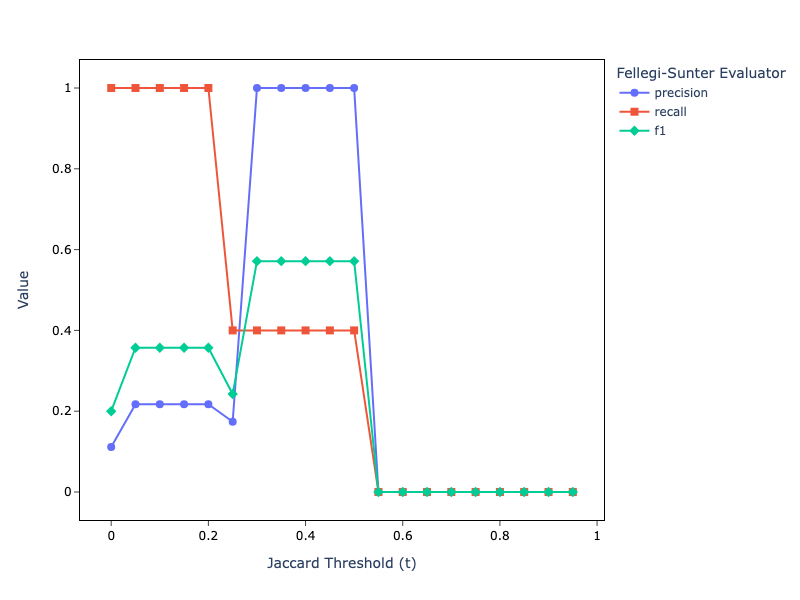
\includegraphics[width=\textwidth]{fellegi-sunter-generated-data}
        \caption{Fellegi-Sunter Results}\label{fsfig}
    \end{figure}

    When the Jaccard similarity threshold is set high ($t \geq 0.66$), we end up
    with few matches, but those matches are true.
    As we lower the threshold ($0.27 \leq t < 0.66$), recall increases and
    precision does not drop.
    However, when we lower the threshold too much ($t < 0.3$) we start losing
    precision and we get better and better recall.
    These results are in line with our expectations.
    So is there anything to learn?

    In our data set we know there are items such as those with the IDs
    208114672 and 208114673.
    These items are near identical and would result in a surplus of matches
    by lowering the Jaccard threshold.
    Lowering the threshold would result in the item with ID 208114672 in Table1
    to be matched with both the item with the same ID in Table2 as well as with
    the item with ID 208114673 from Table2.
    However, all the precision shows us is a resounding 1.
    
    What's more curious is that recall over those same values of \textit{t} is
    not maximal.
    Makes one wonder what's missing.
    While we are working with a simple tiny set of ten items in this experiment,
    imagine working with a large data set.

    Also due to the possible mislabelling of duplicates as true positives we
    seem to get a small rise in precision even as we lower the threshold below
    $0.3$.

    This situation shows us how truly unreliable statistical precision and
    recall can be when judging the output of entity resolution.

    The other thing to notice is the sudden drop in sensitivity around the
    $t=0.3$ mark.
    There is no direct explanation as to why that happens, but it can be assumed
    that since we are also losing duplicated matches, the drop is more
    pronounced than it needs to be.

    \subsection{Algebraic Model}
    The algebraic model represents the ground truth and the entity resolution
    results as partitions over a set containing all the entity references.
    Note that the IDs of the entity references still differ.
    In our catered setup, that means that the input set will contain 20 items.

    In our own setup, the ground truth will contain clusters of two items
    each because of how the data is generated.
    In the `Abt-Buy' setup, all items that are not in the ideal mapping will be
    added as singleton clusters in the ground truth while the items in the ideal
    mapping will be clustered via Kruskall's algorithm using a union-find data
    structure.

    The results are dramatically different from those of the statistical model.

    \begin{figure}
        \begin{minipage}{0.48\textwidth}
            \centering
            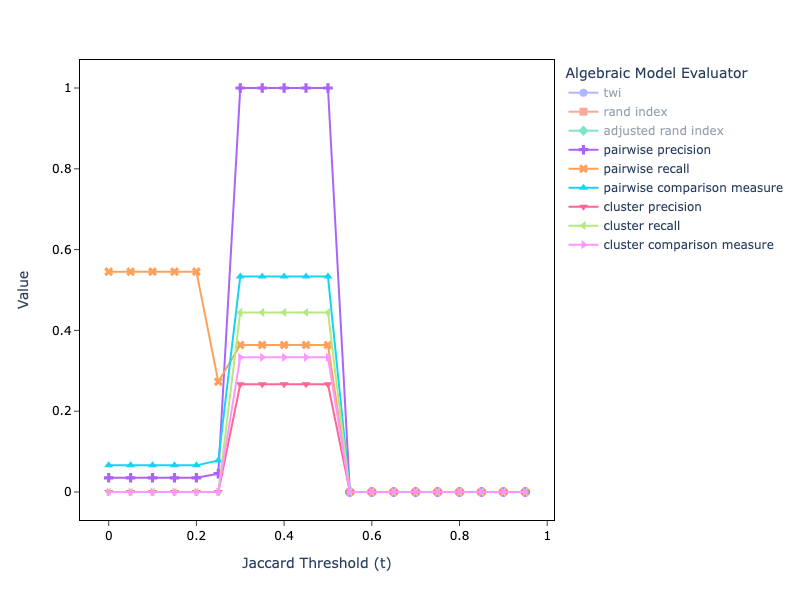
\includegraphics[width=\textwidth]{algebraic-prf-generated-data}
            \caption{Precision, Recall and F1}
        \end{minipage}    
        \begin{minipage}{0.48\textwidth}
            \centering
            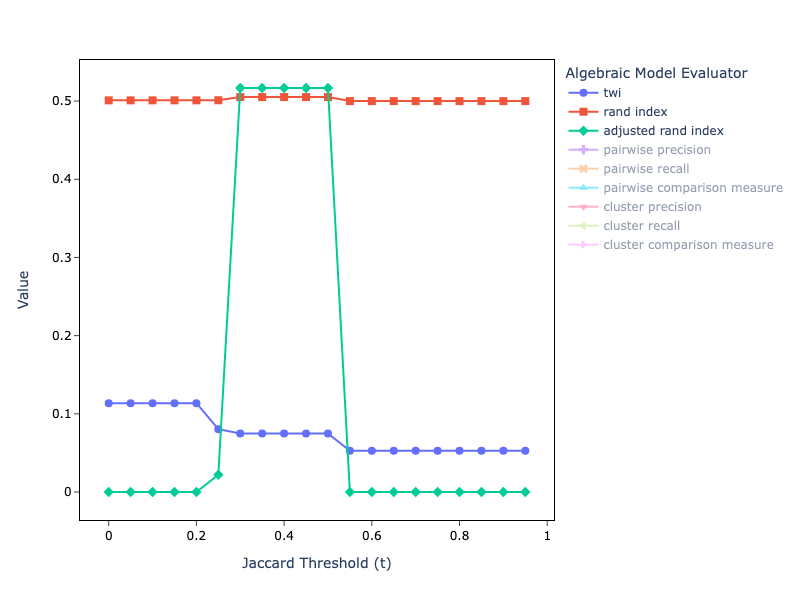
\includegraphics[width=\textwidth]{algebraic-index-generated-data}
            \caption{Clustering Indexes}
        \end{minipage}    
        
    \end{figure}\label{algebraic-prffig}

    The first thing of notice is that there is no bump in precision when we
    lower the $t$ below $0.3$.
    The reason behind this is that the clusters containing near-duplicates will
    not suddenly generate more pairwise combinations than the clusters that
    don't.
    That is, no matter how many times a pairing appears in the list of pairings
    that generates a cluster, the cluster will still contain those two elements.
    It will never include a third.

    Another observation is that we see a very clear signal for $0.3 < t < 0.5$.
    The pairwise precision mimicks what the statistical precision shows us.
    However, the cluster precision tells us that the matching is off by at least
    a half of the size of the input.
    The only way to interpret this is by admitting that the entity resolution
    task duplicates true positives at approximately a 2:1 ratio.
    In our constructed data set, this observation is sustained by the fact that
    8 IDs are very likely to generate what would be extra true positives in the
    statistical approach.

    Concerning recall, we see that cluster recall actually rises along with
    cluster precision.
    This again signals that the pairwise recall we see for $t<0.3$ is most
    likely not worth considering because although a significant proportion of
    the relevant data is returned, a significant proportion of the entity
    profiles constructed are not correct.

    These observations are supported by the additional quality metrics that are
    available via the algebraic model.
    The Rand index and the Adjusted Rand Index confirm the partition lack of
    alignment for $t\notin[0.3,0.5]$, while the Talburt-Wang index confirms that
    more correct pairs are returned as $t$ decreases.

    However, the fundamental takeaway from using the algebraic model is that
    PPJoin does not return near-perfect precision in any case except when taking
    a very narrow view over the pairs of matches it returns.

    
    \subsection{Abt-Buy Results}

    To replicate our results on our own generated data that aimed to exacerbate
    certain data flaws, we run our experiment setup on the `Abt-Buy' data set
    itself.
    
    \section[conclusion]{Conclusions}\label{section:conclusions}

    The work speaks about how we can use mathematical models to evaluate entity resolution results. It also provides easy rules of thumb to identify the model that's best suited to interpret the results of an ER task.
    
    \section[future]{Future Work}\label{section:future}
    \begin{itemize}
        \item result translation between math models
        \item ground truth and data generation for ER tasks
    \end{itemize}


    \bibliographystyle{plain} % We choose the "plain" reference style
    \bibliography{er-general,er-related-work,er-additional-references,er-software}
\end{document}
